%%%%%%%%%%%%%%%%%%%%%%%%%%%%%%%%%%%%%%%%%%%%%%%%%%%%%%%%%%%%%%%%%
% MUW Presentation
% LaTeX Template
% Version 1.0 (27/12/2016)
%
% License:
% CC BY-NC-SA 4.0 (http://creativecommons.org/licenses/by-nc-sa/3.0/)
%
% Created by:
% Nicolas Ballarini, CeMSIIS, Medical University of Vienna
% nicoballarini@gmail.com
% http://statistics.msi.meduniwien.ac.at/
%
% Customized for UAH by:
% David F. Barrero, Departamento de Automática, UAH
%%%%%%%%%%%%%%%%%%%%%%%%%%%%%%%%%%%%%%%%%%%%%%%%%%%%%%%%%%%%%%%%%

\documentclass[10pt,compress]{beamer} % Change 10pt to make fonts of a different size
\mode<presentation>

\usepackage[spanish]{babel}
\usepackage{fontspec}
\usepackage{tikz}
\usepackage{etoolbox}
\usepackage{xcolor}
\usepackage{xstring}
\usepackage{listings}

\usetheme{UAH}
\usecolortheme{UAH}
\setbeamertemplate{navigation symbols}{} 
\setbeamertemplate{caption}[numbered]

%%%%%%%%%%%%%%%%%%%%%%%%%%%%%%%%%%%%%%%%%%%%%%%%%%%%%%%%%%%%%%%%%
%% Presentation Info
\title[Language basics]{Language basics}
\author{}
\institute{\asignatura}
\date{}
%%%%%%%%%%%%%%%%%%%%%%%%%%%%%%%%%%%%%%%%%%%%%%%%%%%%%%%%%%%%%%%%%


%%%%%%%%%%%%%%%%%%%%%%%%%%%%%%%%%%%%%%%%%%%%%%%%%%%%%%%%%%%%%%%%%
%% Descomentar para habilitar barra de navegación superior
\setNavigation
%%%%%%%%%%%%%%%%%%%%%%%%%%%%%%%%%%%%%%%%%%%%%%%%%%%%%%%%%%%%%%%%%

%%%%%%%%%%%%%%%%%%%%%%%%%%%%%%%%%%%%%%%%%%%%%%%%%%%%%%%%%%%%%%%%%
%% Configuración de logotipos en portada
%% Opacidad de los logotipos
\newcommand{\opacidad}{1}
%% Descomentar para habilitar logotipo en pié de página de portada
\renewcommand{\logoUno}{Images/isg.png}
%% Descomentar para habilitar logotipo en pié de página de portada
%\renewcommand{\logoDos}{Images/CCLogo.png}
%% Descomentar para habilitar logotipo en pié de página de portada
%\renewcommand{\logoTres}{Images/ALogo.png}
%% Descomentar para habilitar logotipo en pié de página de portada
%\renewcommand{\logoCuatro}{Images/ELogo.png}
%%%%%%%%%%%%%%%%%%%%%%%%%%%%%%%%%%%%%%%%%%%%%%%%%%%%%%%%%%%%%%%%%

%%%%%%%%%%%%%%%%%%%%%%%%%%%%%%%%%%%%%%%%%%%%%%%%%%%%%%%%%%%%%%%%%
%% FOOTLINE
%% Comment/Uncomment the following blocks to modify the footline
%% content in the body slides. 


%% Option A: Title and institute
\footlineA
%% Option B: Author and institute
%\footlineB
%% Option C: Title, Author and institute
%\footlineC
%%%%%%%%%%%%%%%%%%%%%%%%%%%%%%%%%%%%%%%%%%%%%%%%%%%%%%%%%%%%%%%%%

\begin{document}

%%%%%%%%%%%%%%%%%%%%%%%%%%%%%%%%%%%%%%%%%%%%%%%%%%%%%%%%%%%%%%%%%
% Use this block for a blue title slide with modified footline
{\titlepageBlue
    \begin{frame}
        \titlepage
    \end{frame}
}

\begin{frame}[plain]{}
   \begin{block}{Objective}
       Develop simple algorithms in Java
   \end{block}

   \begin{block}{Bibliography}
      \begin{enumerate}
          \item The Java\textsuperscript{TM} Tutorials. Oracle. \href{https://docs.oracle.com/javase/tutorial/}{(Link)}
      \end{enumerate} 
   \end{block}

\end{frame}

{
\disableNavigation{white}
\begin{frame}[shrink]{Table of Contents}
 \frametitle{Table of Contents}
 \tableofcontents
  % You might wish to add the option [pausesections]
\end{frame}
}

\section{Introduction}
\begin{frame}{Introduction}
	Java is based on the C syntax
		\begin{itemize}
		\item i.e., Java is similar to C
		\end{itemize}
	... however, Java is not C (neither C++)
		\begin{itemize}
		\item Java is Object-Oriented (OO) (classes, interfaces, inheritance, etc)
		\item OOP: Object-Oriented Programming
		\end{itemize}
	Java was designed to be secure and portable
		\begin{itemize}
		\item Intermediate code (bytecode)
		\item Safe execution environment (Java Virtual Machine)
		\item Automatic memory management (no more mallocs)
		\item No pointers in Java (oh yeah!) $\rightarrow$ \alert{Garbage collector}
		\end{itemize}
	If you know C, then you almost know Java
		\begin{itemize}
		\item Variables, operators, expressions and control flow
		\end{itemize}
\end{frame}

\section{Variables}
\subsection{Primitive types}
\begin{frame}{Variables}{Primitive types (I)}
	Warning!: Several names in OOP meaning the same
		\begin{itemize}
		    \item Attribute, fields, member, ...
		\end{itemize}
	Types of variables
		\begin{itemize}
			\item Instance variable (non-static variables): Belongs to the object
			\item Class variable (static variables): Belongs to the class
			\item Local variable: Like in C
			\item Parameters: Do you remember \texttt{public static void main(String[] args)}? That's it
		\end{itemize}

    \begin{columns}
 	   \column{.70\textwidth}
			\begin{block}{Variable related keywords}
				public, protected, private, static, final, new
			\end{block}
	\end{columns}
	\bigskip
	%\item Same naming conventions than C
\end{frame}

\begin{frame}{Variables}{Primitive types (II)}

\centering Variable size is architecture independent
\bigskip
\centering \small{
	%\hspace{-0.7cm}
	\begin{tabular}{cccc} \hline
	\textit{Definition} 	& \textit{Type}		& \textit{Default} 	& \textit{Size} \\\hline
\texttt{byte} 	& Integer	& 0			& 8-bit		\\
\texttt{short} 	& Integer	& 0			& 16-bit 	\\
\texttt{int} 	& Integer	& 0			& 32-bit	\\
\texttt{long} 	& Integer	& 0L		& 64-bit	\\
\texttt{float} 	& Float		& 0.0f		& 32-bit	\\
\texttt{double} & Float		& 0.0d		& 64-bit	\\
\texttt{char} 	& Character	& '$\backslash$u0000'	& 16-bit (Unicode)\\
\texttt{string} & String	& null		& X			\\
\texttt{boolean} & Logic		& false		& 			\\
\hline
\end{tabular}
}
\\
\bigskip
    Same initialization than C: \texttt{int i = 0;}
\end{frame}

\begin{frame}{Variables}{Primitive types (III)}
	\begin{block}{TypesExample.java}
		\lstinputlisting[language=java, basicstyle=\ttfamily\scriptsize]{code/Types.java}
	\end{block}
\end{frame}


\subsection{Arrays}
\begin{frame}{Variables}{Arrays (I)}
	\vspace{-0.2cm}
	An \alert{array} is a sequence of variables of the same type
		\begin{itemize}
		\item The variable is identified by an index
		\item The array length remains constant
		\end{itemize}
	\centering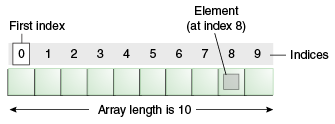
\includegraphics[width=0.5\linewidth]{figs/objects-tenElementArray}\\
    \centering \tiny{\href{http://docs.oracle.com/javase/tutorial/java/nutsandbolts/arrays.html}{(Source)}}

	\vspace{-0.2cm}
	\normalsize{\begin{block}{Example}
	\vspace{-0.2cm}
		\lstinputlisting[language=java, basicstyle=\ttfamily\scriptsize]{code/array-3.java}
	\vspace{-0.2cm}
	\end{block}}
\end{frame}

\begin{frame}{Variables}{Arrays (II)}
	Declaration, creation and initialization are different concepts
	\vspace{-0.2cm}
	\begin{block}{}
	\vspace{-0.2cm}
		\lstinputlisting[language=java, basicstyle=\ttfamily\scriptsize]{code/array-1.java}
	\vspace{-0.2cm}
	\end{block}
\end{frame}

\begin{frame}{Variables}{Arrays (III)}
	The \texttt{main()} function provides the parameters as an array
	\begin{block}{ArrayDemo2.java}
		\lstinputlisting[language=java, basicstyle=\ttfamily\scriptsize]{code/array-2.java}
	\end{block}
\end{frame}

\subsection{Casting}

\begin{frame}{Variables}{Casting}
	We can assign a value to a variable of different type
		\begin{itemize}
		    \item The compiler might guess some converssions
		    \item We can force a conversion: \alert{Casting}
		\end{itemize}
	\begin{block}{CastDemo.java}
	\vspace{-0.2cm}
		\lstinputlisting[language=java, basicstyle=\ttfamily\scriptsize]{code/cast.java}
	\vspace{-0.2cm}
	\end{block}
\end{frame}


\section{Operators}
\subsection{Assignment and aritmetic operators}

\begin{frame}{Operators}{Assignment and arithmetic operators}
    %\vspace{-0.2cm}
    \begin{columns}
    \column{.30\textwidth}
		\centering \begin{tabular}{cl}
		= & Assignment  \\
		+ & Add  		\\
		- & Substration \\
		* & Multiplication \\
		/ & Division 	\\
		\%& Modulus		\\ 
		+= & Assign + 	\\
		-= & Assign - 	\\
		*= & Assign * 	\\
		/= & Assign / 	\\
		\end{tabular}
    \column{.70\textwidth}
		\begin{block}{ArithmeticDemo.java}
		\lstinputlisting[basicstyle=\ttfamily\scriptsize]{code/oper_aritmeticos.java}
		\end{block}
	\end{columns}
\end{frame}

\subsection{Unary operators}

\begin{frame}{Operators}{Unary operators}
    %\vspace{-0.2cm}
    \begin{columns}
    \column{.30\textwidth}
		\centering \begin{tabular}{cl}
		var++ & Increment \\
		var$--$ & Decrement \\
		++var & Increment \\
		$--$var & Decrement \\
		\end{tabular}
    \column{.70\textwidth}
		\begin{block}{UnaryDemo.java}
		\lstinputlisting[language=java, basicstyle=\ttfamily\scriptsize]{code/oper_unary.java}
		\end{block}
	\end{columns}
\end{frame}

\subsection{Relational and conditional operators}

\begin{frame}{Operators}{Relational and conditional operators (I)}
    %\vspace{-0.2cm}
    \begin{columns}
    \column{.35\textwidth}
		\centering \textit{Relational operators}
		\centering \begin{tabular}{cl}
		== &Equal to 	 \\
		!= &Not equal to \\
		>  &Greater than \\
		>= &Great. or eq. to \\
		<  &Less than \\
		<= &Less than or eq. to\\
		\end{tabular}
		
		\bigskip
		\centering \textit{Conditional operators}
		\centering \begin{tabular}{cl}
		\&\& &AND\\
		||	 &OR \\
		! 	 &Negation \\
		\end{tabular}

    \column{.65\textwidth}
		\begin{itemize}
		\item Result: \texttt{true} or \texttt{false} 
			\begin{itemize}
			\item Java supports native boolean variables
			\item The result is a boolean
			\end{itemize}
		\item Widely used in loops and conditions
		\item Truth tables represent the conditional operators
		\end{itemize}

		\centering Truth tables
		\smallskip
    	\begin{columns}
    	\column{.2\textwidth}
    	\column{.3\textwidth}
		\footnotesize{
		\centering \begin{tabular}{c|c}\hline
		A	   &TTFF \\
		B 	   &TFTF \\\hline
		A\&\&B &TFFF \\\hline
		\end{tabular}
		}
    	\column{.3\textwidth}
		\footnotesize{
		\centering \begin{tabular}{c|c}\hline
		A	 &TTFF \\
		B 	 &TFTF \\\hline
		A||B &TTTF \\\hline
		\end{tabular}
		}
    	\column{.2\textwidth}
		\end{columns}
	\end{columns}
\end{frame}

\begin{frame}{Operators}{Relational and conditional operators (II)}
	\begin{block}{ComparisonDemo.java}
		\vspace{-0.2cm}
		\lstinputlisting[language=java, basicstyle=\ttfamily\scriptsize]{code/ComparisonDemo.java}
		\vspace{-0.2cm}
	\end{block}
\end{frame}

\subsection{Bitwise and shift operators}

\begin{frame}{Operators}{Bitwise and shift operators (I)}
    %\vspace{-0.2cm}
    \begin{columns}
    \column{.5\textwidth}
		\centering \textit{Bitwise operators}
		\centering \begin{tabular}{cl}
		\& 	 & Bitwise AND 	\\
		|  	 & Bitwise OR		\\
		{}\^{} & Bitwise XOR\\
		$<<$   & Shift left \\
		$>>$ 	 & Shift right \\
		\~{} & Bit inversion \\
		\end{tabular}

    \column{.65\textwidth}
		\begin{block}{Examples}
    	\begin{columns}
    	\column{.5\textwidth}
		\begin{center}
		AND
		\footnotesize{
		\centering \begin{tabular}{|c|c|}\hline
		A	 &1100 \\
		B 	 &1010 \\
		A\&B &1000 \\\hline
		\end{tabular}
		\normalsize{SHIFT}
		\footnotesize{
		\begin{tabular}{|c|c|}\hline
		A    &1100 \\
		A>>1 &0110 \\\hline
		\end{tabular}
		}
		}
		\end{center}

    	\column{.5\textwidth}
		\begin{center}
		OR
		\footnotesize{
		\begin{tabular}{|c|c|}\hline
		A  &1100 \\
		B  &1010 \\
		A|B&1110 \\\hline
		\end{tabular}\\
		\normalsize{XOR}
		\footnotesize{
		\centering \begin{tabular}{|c|c|}\hline
		A  		&1100 \\
		B  		&1010 \\
		A\^{}B	&0110 \\\hline
		\end{tabular}
		}
		}
		\end{center}
		\end{columns}
		\end{block}
	\end{columns}

	Bit-level operators
		\begin{itemize}
		\item Conditional operators are variable-level
		\end{itemize}
	Classic logic operations
		\begin{itemize}
		\item AND, OR, XOR, shift and inversion
		\item AND is used to put bits to 0
		\item OR is used to put bits to 1
		\end{itemize}
\end{frame}


\begin{frame}{Operators}{Bitwise and shift operators (II)}
		\vspace{-0.2cm}
	\begin{block}{BitDemo.java}
		\vspace{-0.2cm}
		\lstinputlisting[language=java, basicstyle=\ttfamily\scriptsize]{code/BitDemo.java}
		\vspace{-0.2cm}
	\end{block}

	Operations over certain bits: Bitmasks
	\begin{itemize}
	\item Example: Get the value of bit 5
	\end{itemize}

    \begin{columns}
    \column{.3\textwidth}
		\footnotesize{
		\begin{tabular}{cc}
		xxx1xxxx & \& \\
		00010000 & =  \\
		----------- &    \\
		00010000 &    \\
		\end{tabular}
		}
 	\column{.3\textwidth}
		\footnotesize{
		\begin{tabular}{cc}
		xxx0xxxx & \&  \\
		00010000 & =   \\
		----------- &     \\
		00000000 &     \\
		\end{tabular}
		}
	\end{columns}
\end{frame}

\section{Control flow}
\subsection{Control flow introduction}
\begin{frame}{Control flow}{Control flow introduction}
    %\vspace{-0.2cm}
	Control flow breaks up the flow of execution
	\begin{itemize}
	\item Conditions (if-then, switch)
	\item Loops (for, while, do-while)
	\item Branching (break, continue, return)
	\end{itemize}
    Usually used with code blocks
\end{frame}

\subsection{Blocks}

\begin{frame}{Control flow}{Blocks}
	\vspace{-0.2cm}
	A block is a group of statements between braces (``\{'' y ``\}'')
	    \begin{itemize}
		\item A block is a unity of code
		\item Braces never end with semicolon (``;'')
		\item Used with loops, methods, conditions, etc
	    \end{itemize}

	\vspace{-0.2cm}
    \begin{columns}
    \column{.15\textwidth}
    \column{.30\textwidth}
	\footnotesize{
		\begin{block}{}
		\lstinputlisting[language=java, basicstyle=\ttfamily\scriptsize]{code/bloques-1.c}
		\end{block}
	}
    \column{.05\textwidth}
		\alert{\Large{$\ne$}}
    \column{.30\textwidth}
	\footnotesize{
		\begin{block}{}
		\lstinputlisting[language=java, basicstyle=\ttfamily\scriptsize]{code/bloques-2.c}
		\end{block}
	}
    \column{.15\textwidth}
	\end{columns}
	
	\vspace{-0.2cm}
    \begin{columns}
    \column{.7\textwidth}
		 A variable can be defined at block-level
			\begin{itemize}
			\item The variable only exists within the block
			\item Good practice: Limiting the scope of the variables
	    	\end{itemize}
    \column{.3\textwidth}
		\begin{block}{}
		\lstinputlisting[language=java, basicstyle=\ttfamily\scriptsize]{code/bloques-3.c}
		\end{block}
	\end{columns}

\end{frame}

\subsection{Conditional statements}

\begin{frame}{Control flow}{Conditional statements: if-else statement (I)}
	Conditional statements implement decision making
    \begin{itemize}
		\item They are based on a conditional statement
		\item The result is a boolean
		\item Remember: Java supports a booleans!
    \end{itemize}

	\vspace{-0.2cm}
    \begin{columns}
    \column{.05\textwidth}
    \column{.40\textwidth}
	\footnotesize{
		\begin{block}{}
		\vspace{-0.2cm}
		\lstinputlisting[language=java, basicstyle=\ttfamily\scriptsize]{code/if-1.c}
		\vspace{-0.2cm}
		\end{block}
	}
   	\column{.05\textwidth}
		\Large{$\approx$}
    \column{.40\textwidth}
	\footnotesize{
		\begin{block}{}
		\vspace{-0.2cm}
		\lstinputlisting[language=java, basicstyle=\ttfamily\scriptsize]{code/if-2.c}
		\vspace{-0.2cm}
		\end{block}
	}
    \column{.05\textwidth}
	\end{columns}
	\begin{center} Good practice: The usage of \texttt{else} is optional, try to avoid it! \end{center}
\end{frame}

\begin{frame}{Control flow}{Conditional statements: if-else statement (II)}
	\vspace{-0.2cm}
    \begin{columns}
    \column{.6\textwidth}
		\begin{itemize}
		\item Many times decisions are not binary (true/false)
		\item Grouped conditions
			\begin{itemize}
			\item Conditions are evaluated until first true
			\item If all conditions are false, then it executes \texttt{else}
			\item \texttt{else} is optional (try not to use it!)
			\end{itemize}
	    \end{itemize}
    \column{.4\textwidth}
		\begin{block}{}
		\vspace{-0.2cm}
		\lstinputlisting[language=java, basicstyle=\ttfamily\scriptsize]{code/elseif-1.c}
		\vspace{-0.2cm}
		\end{block}
    %\column{.1\textwidth}
	\end{columns}
\end{frame}

\begin{frame}{Control flow}{Conditional statements: if-else statement (III)}
	\vspace{-0.4cm}
	\begin{columns}
	\column{\textwidth}
	\small{
	\begin{block}{Example}
		\vspace{-0.25cm}
		\lstinputlisting[language=java, basicstyle=\ttfamily\scriptsize]{code/elseif-2.c}
		\vspace{-0.2cm}
	\end{block}
	}
	\end{columns}
\end{frame}

\begin{frame}{Control flow}{Conditional statements: Ternary operator (IV)}
	The statement \texttt{if} ... \texttt{else} is pretty common 
    \begin{itemize}
		\item Sometimes to simply assign a variable value
		\item It makes code hard to read
    \end{itemize}
	Ternary operator: \texttt{condition? if-true : if-false;}
	\vspace{-0.2cm}
    \begin{columns}
    \column{.05\textwidth}
    \column{.40\textwidth}
	\footnotesize{
		\begin{block}{}
		\vspace{-0.2cm}
		\lstinputlisting{code/ternary-1.c}
		\vspace{-0.2cm}
		\end{block}
	}
   	\column{.05\textwidth}
		\Large{=}
    \column{.40\textwidth}
	\footnotesize{
		\begin{block}{}
		\vspace{-0.2cm}
		\lstinputlisting{code/ternary-2.c}
		\vspace{-0.2cm}
		\end{block}
	}
    \column{.05\textwidth}
	\end{columns}
\end{frame}


\begin{frame}{Control flow}{Conditional statements: switch (I)}
	\vspace{-0.2cm}
    \begin{columns}
    \column{.6\textwidth}
		\begin{itemize}
		\item Closely related to \texttt{if else}
			\begin{itemize}
			\item Sometimes \texttt{switch} is more convenient
			\end{itemize}
		\item It evaluates an expression and, depending on its result, takes a branch
		\item There is a \texttt{default} action
		\item The keyword \texttt{break} exits the statement
	    \end{itemize}
    \column{.4\textwidth}
		\begin{block}{}
		\vspace{-0.2cm}
		\lstinputlisting[language=java, basicstyle=\ttfamily\scriptsize]{code/switch-1.c}
		\vspace{-0.2cm}
		\end{block}
    %\column{.1\textwidth}
	\end{columns}
\end{frame}

\begin{frame}{Control flow}{Conditional statements: switch (II)}
	\vspace{-0.4cm}
	\begin{columns}
	\column{0.7\textwidth}
	\begin{block}{Example}
		\vspace{-0.25cm}
		\lstinputlisting[language=java, basicstyle=\ttfamily\scriptsize]{code/switch-2-a.c}
		\vspace{-0.2cm}
	\end{block}
	\end{columns}
\end{frame}

\subsection{Loops}

\begin{frame}{Control flow}{Loop statements: for and while (I)}
	\texttt{For} and \texttt{while} are the two most common loop statements
	\vspace{-0.2cm}
    \begin{columns}
    %\column{.05\textwidth}
    \column{.50\textwidth}
	\footnotesize{
		\begin{block}{for syntax}
		\vspace{-0.2cm}
		\lstinputlisting{code/bucles-1.c}
		\vspace{-0.2cm}
		\end{block}
	}	
    \column{.05\textwidth}
		\Large{=}
    \column{.40\textwidth}
	\footnotesize{
		\begin{block}{while syntax}
		\vspace{-0.2cm}
		\lstinputlisting{code/bucles-2.c}
		\vspace{-0.2cm}
		\end{block}
	}
    \column{.05\textwidth}
	\end{columns}

	\begin{itemize}
	\item The statements \texttt{for} and \texttt{while} are equivalents
	\item The \texttt{for} statement can be read as
		\begin{itemize}
		\item For \texttt{expr1}, while \texttt{expr2}, do \texttt{expr3}
		\end{itemize}
    \end{itemize}
\end{frame}

\begin{frame}{Control flow}{Loops: iterating collections}
	\vspace{-0.2cm}
	\begin{block}{Old syntax}
	\vspace{-0.2cm}
	\lstinputlisting[language=java, basicstyle=\ttfamily\scriptsize]{code/DemoFor2.java}
	\vspace{-0.2cm}
	\end{block}

	\vspace{-0.2cm}
    \begin{block}{Modern syntax (> Java 5)}
	\vspace{-0.2cm}
	\lstinputlisting[language=java, basicstyle=\ttfamily\scriptsize]{code/DemoFor.java}
	\vspace{-0.2cm}
	\end{block}
\end{frame}

\begin{frame}{Control flow}{Loops: do-while (I)}
    \begin{columns}
    %\column{.05\textwidth}
    \column{.50\textwidth}
		Statements \texttt{for} y \texttt{while} assess first
			\begin{itemize}
			\item Execution is not assured
			\end{itemize}
		Statement do-while first executes, then assesses
			\begin{itemize}
			\item The body is executed at least one time
			\item Some times, using a do-while saves code
			\end{itemize}
	    It can be read as ``do ... while ...''
    \column{.50\textwidth}
		\begin{block}{do-while syntax}
		\vspace{-0.2cm}
		\lstinputlisting[language=java, basicstyle=\ttfamily]{code/dowhile-1.c}
		\vspace{-0.2cm}
		\end{block}
    \column{.05\textwidth}
	\end{columns}
\end{frame}

\begin{frame}{Control flow}{Loops: do-while (II)}
	\begin{columns}
	\column{\textwidth}
	\begin{block}{Example}
		\lstinputlisting[language=java, basicstyle=\ttfamily\scriptsize]{code/dowhile-2.c}
	\end{block}
	\end{columns}
\end{frame}

\subsection[Branching statements]{Branching statements}

\begin{frame}{Control flow}{Branching statements: Break and continue (I)}
	\begin{itemize}
	\item \texttt{break}: Exit the loop
	\item \texttt{continue}: Jump to next iteration
	\item \texttt{break} and \texttt{continue} are valids in loops
	\begin{itemize}
	\item \texttt{break} can be used, in addition, in a \texttt{switch} statement
	\end{itemize}
	\end{itemize}
	\vspace{-0.2cm}
    \begin{columns}
    \column{.50\textwidth}
	\footnotesize{
		\begin{block}{Example: break}
		\vspace{-0.2cm}
		\lstinputlisting{code/break-1.java}
		\vspace{-0.2cm}
		\end{block}
	}
    \column{.50\textwidth}
	\footnotesize{
		\begin{block}{Example: Continue}
		\vspace{-0.2cm}
		\lstinputlisting{code/continue-1.java}
		\vspace{-0.2cm}
		\end{block}
	}
	\end{columns}
\end{frame}

\begin{frame}{Control flow}{Branching statements: Break and continue (II)}
	\vspace{-0.3cm}
	\begin{columns}
	\column{\textwidth}
	\begin{block}{Break example}
	\vspace{-0.2cm}
		\lstinputlisting[language=java, basicstyle=\ttfamily\scriptsize]{code/break-2.java}
	\end{block}
	\end{columns}
	Exercise: Use loops modern syntax
\end{frame}

\begin{frame}{Control flow}{Branching statements: Break and continue (III)}
	\vspace{-0.3cm}
	\begin{columns}
	\column{\textwidth}
	\small{
	\begin{block}{Continue example}
		\lstinputlisting[language=java, basicstyle=\ttfamily\scriptsize]{code/continue-2.c}
	\end{block}
	}
	\end{columns}
\end{frame}

\end{document}

\begin{frame}{Control flow}{Conditional statements}
    \begin{columns}
    \column{.5\textwidth}
%		\begin{block}{Operador ternario}
%		\texttt{condicion? si-verdadero : si-falso;}
%		\end{block}

		\begin{itemize}
			\item Conditional statements are everywhere
			\item Ternary operator simplifies the code
		\end{itemize}

    \column{.5\textwidth}
	\begin{itemize}
	\item This code
		\lstinputlisting{code/oper_ternario-1.c}
	\item is equivalent to
		\lstinputlisting{code/oper_ternario-2.c}
	\item It can be used in complex expressions
		\lstinputlisting{code/oper_ternario-3.c}
	\end{itemize}
	\end{columns}
\end{frame}



\end{document}
